\chapter{三维重建的一般方法以及改进}
\label{cha:chap3}
\section{引言}
\label{sec:3.1}
内容内容内容内容内容内容内容内容内容内容内容内容内容内容内容
\section{三维重建的一般步骤}
\label{sec:3.2}
三维重建是指从三维图像中复原三维场景或者物体的过程,整个流程的输入为无序的图片即可,输出可以得到三维重建后的稀疏点云和稠密
点,大致流程如图~\ref{fig:3Dconstr_pipiline_sfm}所示。
\begin{figure}[H] % use float package if you want it here
    \centering
    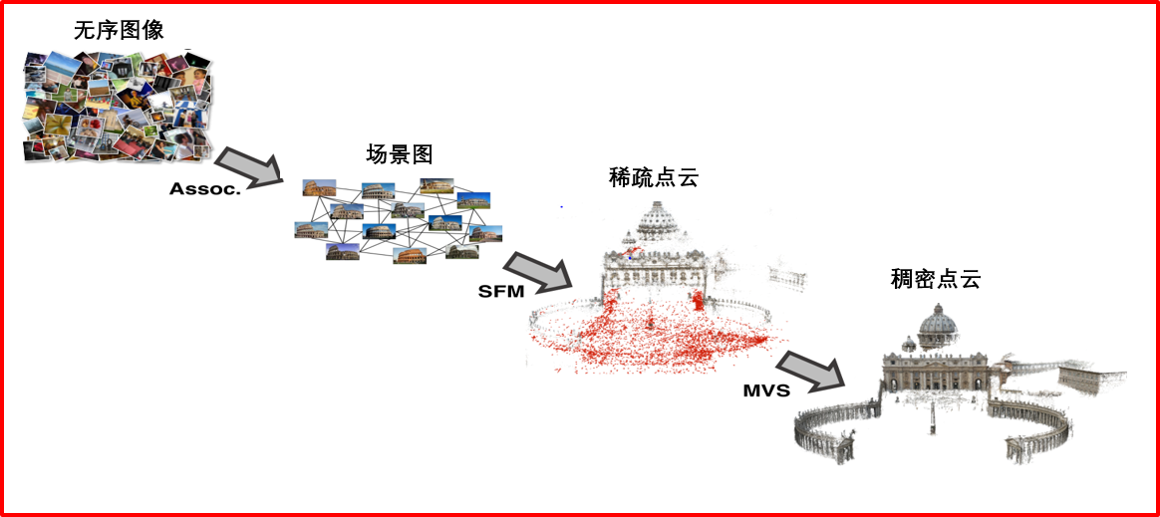
\includegraphics[width=12cm]{3Dconstr_pipiline_sfm.png}
    \caption{三维重建流程图}
    \label{fig:3Dconstr_pipiline_sfm}
    \end{figure}
\subsection{一般方法概述}
\label{sec:3.2.1}
对于以上流程进一步进行细化,整个三维重建的过程可以划分为以下几个主要的步骤:

1.  2D图像采集:多角度拍摄或者从视频中提取到一组图像序列,将图像序列作为整个系统的输入;

2.  特征点提取和匹配:根据拍摄到的图像,提取每张图像之间的特征点,并进行特征点的匹配;

3.  稀疏点云:根据匹配结果估计特征点的深度,提取出稀疏点云,并估计相机的位姿和参数;

4.  稠密点云:根据优化后的相机参数和匹配结果,获得稠密点云;

5.  纹理映射:根据以上点重建物体表面,进行纹理映射。

三维重建的一般步骤可以简化为如图~\ref{fig:3Dconstr_pipiline}所示。
\begin{figure}[H] % use float package if you want it here
    \centering
    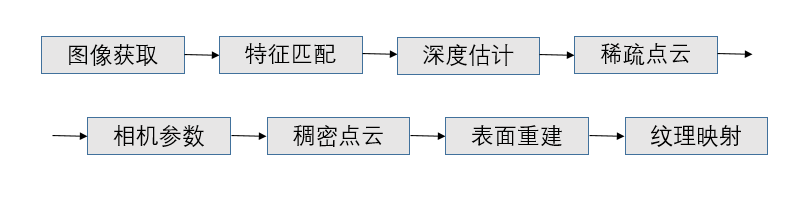
\includegraphics[width=12cm]{3Dconstr_pipiline.png}
    \caption{三维重建一般步骤流程图}
    \label{fig:3Dconstr_pipiline}
    \end{figure}

三维重建主要分为多个步骤,目前很多开源的系统都可以完成其中的部分环节,对于完整的三维重建流程还需要多个系统相互连接实现,
表~\ref{tab:3D_compare}是当前三维重建系统的简要对比。本文在考虑到各个系统流程的完整性和合理性,以及在实际测试过系统之
间的效果差异后,选择Colmap作为作为三维重建的工具。
\begin{table}[h]
    \centering
    \caption{常见三维重建系统对比表}
    \label{tab:3D_compare}
    \begin{tabular}{C{3.6cm}C{2.4cm}C{2.4cm}C{2.4cm}C{2.4cm}}
    \toprule
    \textbf{系统名称} & \textbf{稀疏点云} &\textbf{稠密点云} &  \textbf{重建表面} &\textbf{纹理映射}  \\
    \midrule
    Bundler       &\cellcolor{green}是&\cellcolor{gray}否&\cellcolor{gray}否&\cellcolor{gray}否\\
    CMVS          &\cellcolor{gray}否&\cellcolor{green}是&\cellcolor{gray}否&\cellcolor{gray}否\\
    Colmap        &\cellcolor{green}是&\cellcolor{green}是&\cellcolor{green}是&\cellcolor{gray}否\\
    Meshlab       &\cellcolor{gray}否&\cellcolor{gray}否&\cellcolor{green}是&\cellcolor{green}是\\
    MVE           &\cellcolor{green}是&\cellcolor{green}是&\cellcolor{green}是&\cellcolor{gray}否\\
    MVS-texturing &\cellcolor{green}是&\cellcolor{green}是&\cellcolor{green}是&\cellcolor{gray}否\\
    openMVG       &\cellcolor{green}是&\cellcolor{green}是&否\cellcolor{gray}&\cellcolor{gray}否\\
    openMVS       &\cellcolor{gray}否&\cellcolor{gray}否&\cellcolor{green}是&\cellcolor{green}是\\
    Theia         &\cellcolor{green}是&\cellcolor{gray}否&\cellcolor{gray}否&\cellcolor{gray}否\\
    VisualFSM     &\cellcolor{green}是&\cellcolor{green}是&\cellcolor{gray}否&\cellcolor{gray}否\\
    \bottomrule
    \end{tabular}
  \end{table}
\subsection{三维重建详细过程解析}
\label{sec:3.2.2}
\subsubsection{图像获取} 
\label{sec:3.2.2.1}
目前常规的三维重建仅需要输入无序图片,在构图的过程中,可以极大地降低操作的复杂度,并且对于相机的内参和外参也无需提前提供给整
个三维重建的系统,在特征点匹配的过程中,这些参数都可以通过计算得到。对于输入的图像,可以通过随着时间流单帧拍摄的方式获取或者
通过截取视频流的方式得到,且图像之间不能仅有纯旋转,这样无法估计深度。在获取图像的过程中,需要注意保证每连续两帧图像之间尽可
能保证30$\%$的重叠区域,相邻两帧之间的旋转角度为30度到45度之间,且物体中的每一个点至少能被三帧图像观测到。
\subsubsection{特征点的检测和匹配} 
\label{sec:3.2.2.2}
目前,在三维重建领域中图像的特征匹配就是以特征点为基础而进行的,所以,如何定义和找出一幅图像中的特征点就非常重要。常见的
特定点检测和匹配主要包括SUFT,SIFT,ORB,Harris角点等,各方法的简要特点如表所示。
\begin{table}[h]
    \centering
    \caption{常见特征检测方法对比表}
    \label{tab:Feature}
    \begin{tabular}{C{4.6cm}L{8.4cm}}
    \toprule
    \textbf{方法名称} & \textbf{特点}  \\
    \midrule
    SUFT&解决特征检测中的尺度不变性问题,具备较高的计算效率\\
    SIFT&以SUFT为基础,基于浮点内核计算特征点,有着更加精确的空间位置和尺度\\
    ORB&满足实时性的速度,但是不具备旋转,尺度不变性且噪声敏感\\
    Harris角点&能够较好的检测角点,进行精确的定位\\
    \bottomrule
    \end{tabular}
  \end{table}

对于本文中的三维重建,选择SIFT作为特征点的检测和匹配方法,针对其计算耗时的问题,本文选择CUDA进行硬件加速,另外还考虑到三维
重建本身是一个离线处理的过程,对算法的实时性没有过高要求。SIFT和其他方法相比较,有以下优点:\\
1. SIFT特征是图像的局部特征,其对旋转、尺度缩放、亮度变化保持不变性,对视角变化、仿射变换、噪声也保持一定程度的稳定性;\\
2. 独特性好,信息量丰富,适用于在海量特征数据库中进行快速、准确的匹配;\\
3. 多量性,即使少数的几个物体也可以产生大量的SIFT特征向量。\\
如图~\ref{fig:3Dconstrmatchresult}所示,分别对两帧图形提取SIFT特征,随后根据特征点进行匹配。
\begin{figure}[H]
    \centering
      \subcaptionbox{第1帧图像提取SIFT特征}{\label{fig::3Dconstr_a}
      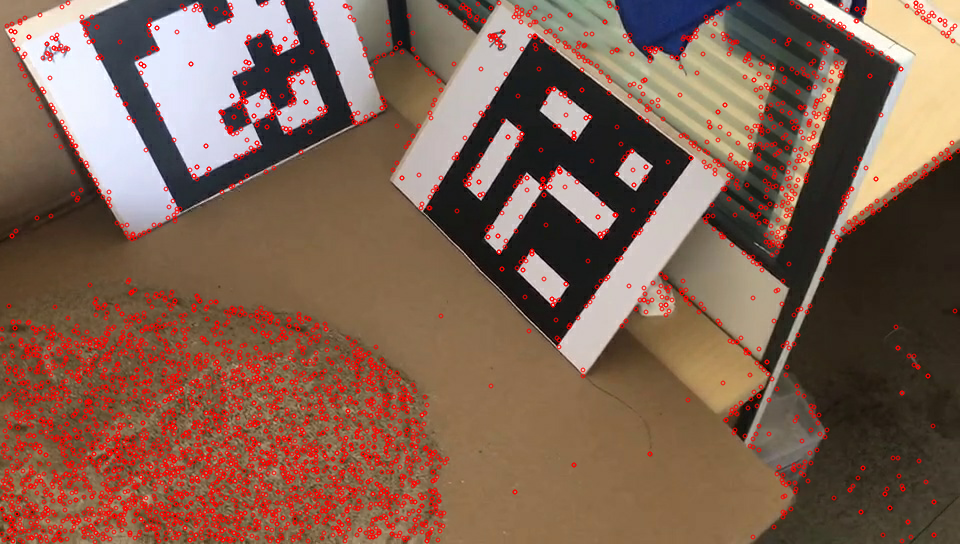
\includegraphics[width=6cm]{3Dconstr_a.png}\hskip2cm}
      \subcaptionbox{第2帧图像提取SIFT特征}{\label{fig:3Dconstr_b}
      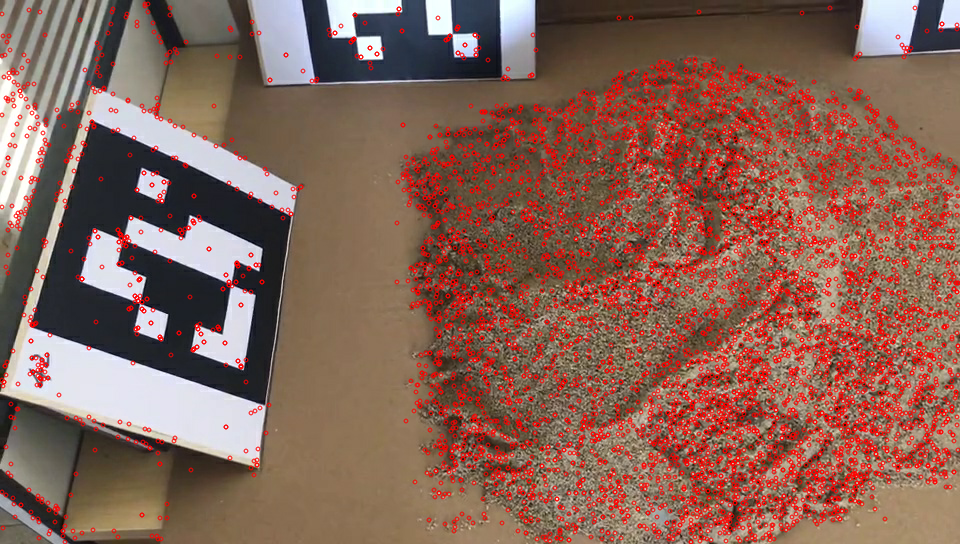
\includegraphics[width=6cm]{3Dconstr_b.png}}
    \vskip0.5cm
      \subcaptionbox{根据特征点进行匹配\label{fig:chap03:3Dconstr_match}}{
      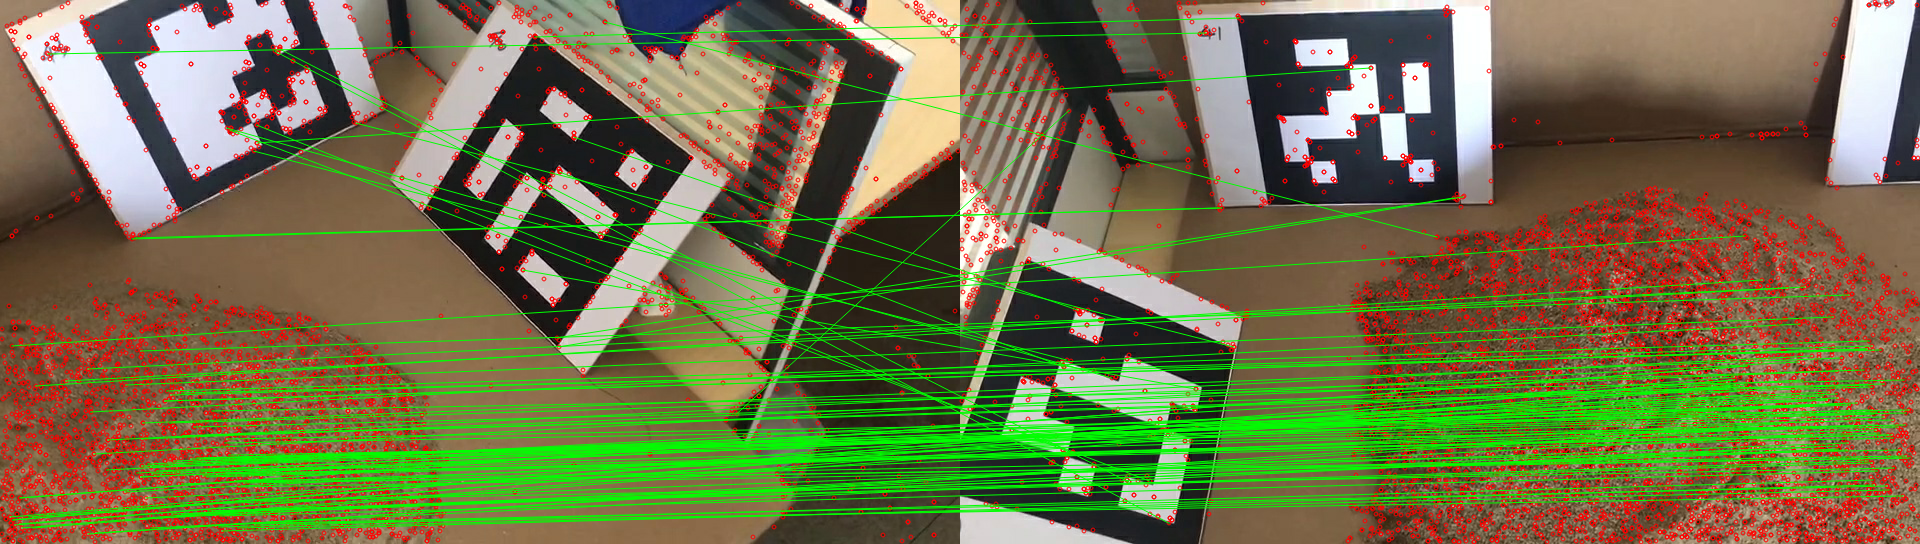
\includegraphics[width=12cm]{3Dconstr_match.png}\hskip2cm}
    \caption{特征提取与匹配结果示意图}\label{fig:3Dconstrmatchresult}
  \end{figure}
在获取到每张图像上的特征点后,需要对图像之间建立匹配关系,常用的方式可以采用计算欧式距离的办法:1)完全匹配,对所有的特征
点都进行穷举,计算其对应距离。2)邻近搜索,建立KD树,缩小搜索范围,能提高效率,但也有可能不是最优,所以邻域取值是关键,越大越准
确,越大计算量越大。由图~\ref{fig:chap03:3Dconstr_match}~所示,两帧之间大多数特征点都可以正确匹配,但依然存在存在部分匹配
是错误的,在本文中,选择了RANSAC(随机抽样一致性)的方式来剔除错误的匹配对,以更加准确的估计相机位姿,RANSAC是指可以从一组
包括局外点(错误匹配)的观测数据中,通过迭代的方式估计数学模式中的参数,通过RANSAC处理后的匹配结果如
图~\ref{fig:3Dconstr_matchAfterRansac}所示,误检的匹配已经被明显的降低。
\begin{figure}[H] % use float package if you want it here
  \centering
  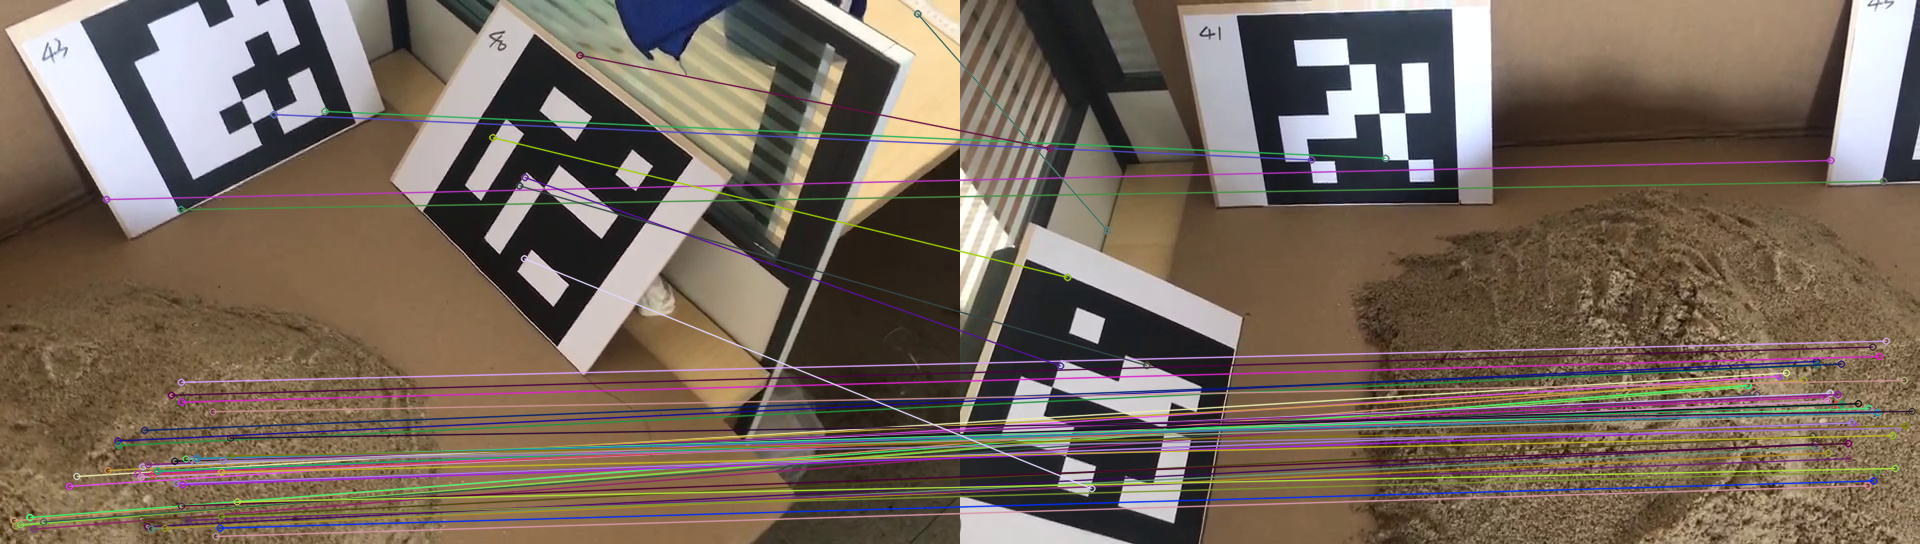
\includegraphics[width=12cm]{3Dconstr_matchAfterRansac.png}
  \caption{RANSAC之后的点云匹配}
  \label{fig:3Dconstr_matchAfterRansac}
  \end{figure}
\subsubsection{SfM} 
\label{sec:3.2.2.3}
在~\ref{sec:3.2.2.2}小节中,可以获得初始的匹配关系,但是这种匹配关系不完全可靠,需要添加几何约束进行检测,该集合约束完全依
赖于场景中的客观事实。可以通过基本矩阵F将匹配好的两帧图像之间的像素坐标(x,y),(x',y')进行关联,假设一个符合条件的匹配对像素坐标需要满足以
下公式:
\begin{equation}
\begin{bmatrix}x'&y'&z'\end{bmatrix}\mathrm F\begin{bmatrix}\mathrm x\\\mathrm y\\\mathrm z\end{bmatrix}=0
\end{equation}

找到相机基线最大的像对,根据该像对,通过RANSC八点法计算本征矩阵,再通过对本征矩阵SVD分解得到第二个图像的R、T,在这一步需要进行畸变校正,
然后根据R、T和矫正后的像点坐标三角计算出三维点。

当所有的两两匹配图像对被确定以后,可以开始计算相机的位姿(3*3的旋转矩阵R,1*3的平移向量t),摄像机的内参(焦距f,畸变参数
k1,k2)。几何场景提供轨迹中的每个3D点$X_j$,通过投影方程,将3D点投影到摄像机的2D成像平面上,投影误差的定义为投影点和图像上
真实点之间的欧式距离,如图~\ref{fig:3Dconstr_reprojection-error}所示。
\begin{figure}[H] % use float package if you want it here
  \centering
  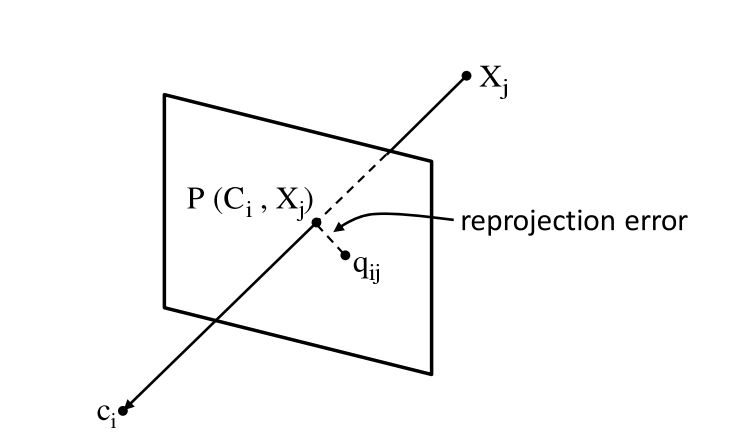
\includegraphics[width=12cm]{3Dconstr_reprojection-error.png}
  \caption{误差投影示意图}
  \label{fig:3Dconstr_reprojection-error}
\end{figure}
对于n个视角和m个轨迹,投影误差的目标优化方程为:
\begin{equation}
  \mathfrak g(C,X)=\sum_{i=1}^n\sum_{j=1}^m\omega_{ij}\left|\left|q_{ij}-P(C_i,X_j)\right|\right|^2
\end{equation}
其中$\left|\left|q_{ij}-P(C_i,X_j)\right|\right|^2$就是摄像机i中的轨迹j的投影误差累积和,SFM算法的目标就是找到合适的相机
和场景参数去优化这个目标函数,g是采用一个非线性最小二乘的优化方法求解,常用BA(光束平差法)来优化上述过程。
最后,不断添加新的摄像机和3D点进行BA。这个过程直到剩下的摄像机观察到的点不超过20为止,说明剩下的摄像机没有足够的点可以添加,
BA结束。得到相机估计参数和场景几何信息,即稀疏的3D点云。
\subsection{当前三维重建存在的问题}
\label{sec:3.2.3}
根据~\ref{sec:3.2}节的描述,可以发现通过现有的三维重建技术流程可以实现有多张连续图像到三维点云的转化,整个过程操作起来十分
简便,且能够得到一个较好的结果。但是从整体实验速度,三维点云结果的精确性来看,依然还存在很多的问题:\\
1. 整个三维重建的过程十分耗时,由于三维重建中的图像时间没有时序信息,关键帧之前的匹配都通过完全枚举的方式进行匹配,对于输入
N张原始图像的系统,时间复杂度高达O($N^2$),由单帧图像到稀疏点云一般耗时为几分钟,由单帧图像到稠密点云耗时耗时更是会高度几
个小时。\\
2. 独三维点云的精度不高,噪音点较大,一方面是由于三维重建往往采取增量式的重建方式,导致最终场景重建的结果无法闭合;另外一方
面也是由于对于某些重复度较高的场景,关联帧之间的匹配由于缺少时序信息,从而导致匹配精度较低,在解算相机位姿时,得到的结果也无
法保证正确,如图~\ref{fig:chap2:3dconstr_stone}所示。
\begin{figure}[htbp]
  \centering
    \subcaptionbox{正面}{\label{fig:chap1:3dconstr_stone1}
    \includegraphics[width=4cm,height=5cm]{3dconstr_stone1.JPG}}
    \subcaptionbox{斜侧面}{\label{fig:chap1:3dconstr_stone2}
    \includegraphics[width=4cm,height=5cm]{3dconstr_stone2.JPG}}
    \subcaptionbox{侧面}{\label{fig:chap1:3dconstr_stone3}
    \includegraphics[width=4cm,height=5cm]{3dconstr_stone3.JPG}}
  \vskip0.5cm
  \subcaptionbox{无法闭合}{\label{fig:chap1:3Dconstr_stone1}
  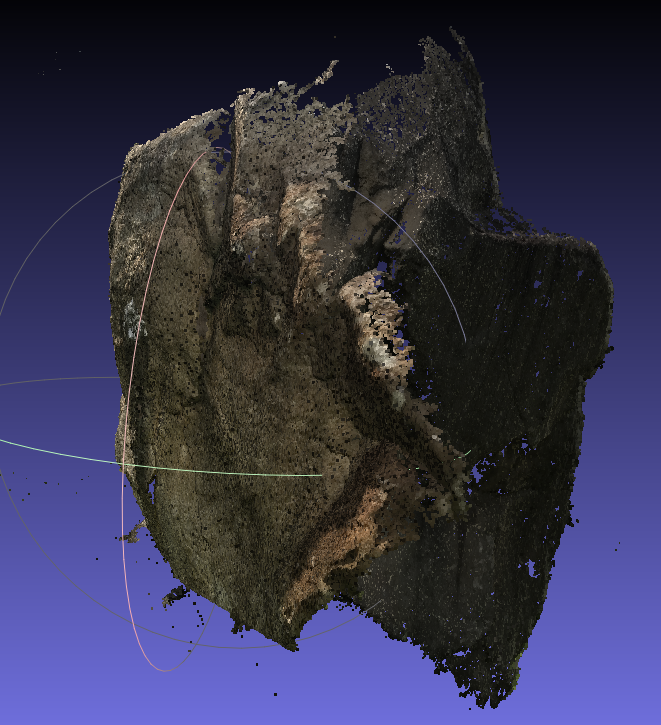
\includegraphics[width=4cm,height=5cm]{3Dconstr_stone1.png}}
  \subcaptionbox{缺失较多}{\label{fig:chap1:3Dconstr_stone2}
  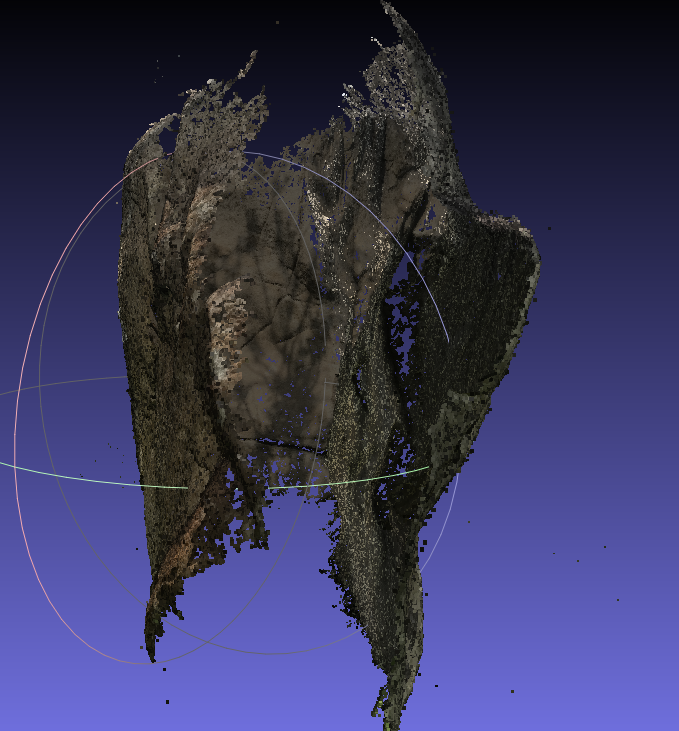
\includegraphics[width=4cm,height=5cm]{3Dconstr_stone2.png}}
  \subcaptionbox{噪音点多}{\label{fig:chap1:3Dconstr_stone3}
  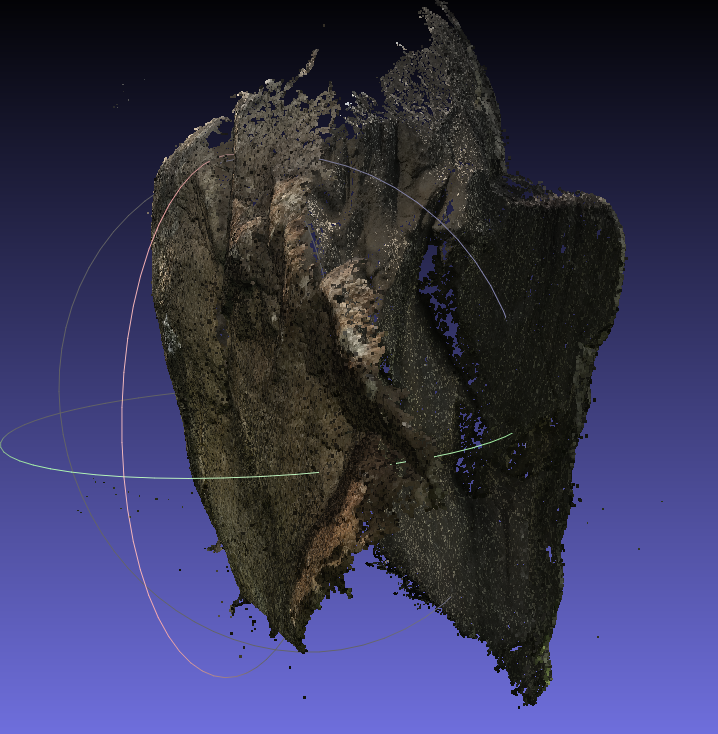
\includegraphics[width=4cm,height=5cm]{3Dconstr_stone3.png}}
  \caption{自然场景三维重建结果示意图}\label{fig:chap2:3dconstr_stone}
\end{figure}
\section{三维重建的优化讨论}
\label{sec:3.3}
\subsection{增加实效性方案}
\label{sec:3.3.1}
在对无序的图像进行三维重建时,会有大量的时间耗费在图像的匹配过程中,在三维重建中常见的图像匹配方法以下几种方法:

1.  完全匹配:当用于三维重建的图像数量较低时,这种匹配模式一般可以较快的完成,并且产生一个比较好的匹配结果,在这种模式里,
每一帧图像都会和其他所有的图像进行匹配验证。但是一旦图像的数量较大,那么这种图形匹配方式将极其耗时,延缓整个三维重建的实效
性。

2.  序列匹配:该匹配模式一般用于图像帧是连续获取得到的情况下,连续的两帧之间就会存在视觉重叠部分,这样的话就不需要对所有帧
进行完全匹配,只需要考虑前后帧即可。

3.  空间匹配:该匹配模式会考虑到每一帧图像的空间位置,通过空间位置这一指标获取到和其相邻的匹配帧,每一帧的空间位置可以认为
设定,或者通过图像自带的GPS信息获取,该模式会对提供的图像空间位置要求较高。

4.  传递匹配:当确定帧A和帧B都和帧C有匹配关系时,那么就默认帧A和帧B也具备匹配关系,这样的匹配模式实效性较快,但是误差较大,
且匹配数量也较高。

5.  自定义匹配:即完全在系统进行匹配查找时就将所有的匹配关系自定义的给出,以自定义的匹配结果代替三维重建中的匹配方法。

对于上述几种三维重建中的使用得当匹配方法,需要同时考虑到匹配时效和匹配精度的问题。排除空间匹配的方法,因为在密闭的环境中很难
获取到每一帧图像所对应的真实GPS信息,对于每帧图像所自带的EXIF信息也会受到GPS强弱的影响,此外通过无人机获取到得到图像,即使
有两帧之间的空间位置十分接近,也无法保证两帧图像具备匹配关系,例如在无人机正反来回的的两帧即使空间位置十分接近,也不一定是匹
配帧。

对于自定义的匹配模式,本文将选择SLAM的结果提供给三维重建进行图像匹配,即将有序化的图像输入代替无序化的图像输入,一方面可以
避免完全匹配带来的耗时问题,同时具备时序信息的SLAM所产生的匹配结果更加精确,鲁棒性更强。对于具体的实现过程,以连续视频流作
为SLAM系统的输入,筛选出其中的关键帧和所有关键帧之间的对应关系,将SLAM中的关键帧作为三维重建的图像输入,关键帧之间的匹配关
系作为三维重建的先验匹配结果,具体流程如图~\ref{fig:3Dconstr_SLAM_pipeline}所示。
\begin{figure}[H] % use float package if you want it here
  \centering
  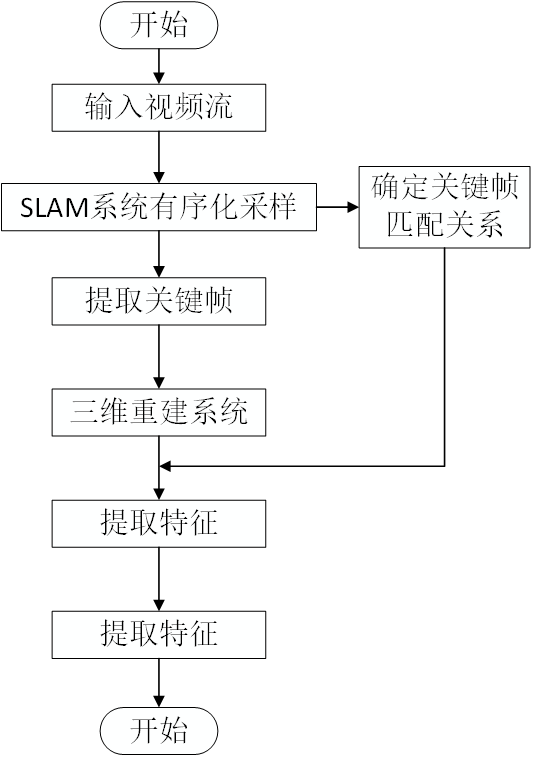
\includegraphics[height=8cm]{3Dconstr_SLAM_pipeline.png}
  \caption{融合SLAM结果的三维重建流程图}
  \label{fig:3Dconstr_SLAM_pipeline}
\end{figure}
本文将说明SLAM中关键帧的提取策略和关键帧之间的匹配策略。首先关键帧相当于SLAM的框架,是在局部一系列普通帧中选出一帧作为局部帧
的代表,记录局部信息,但相机在场景中的某个区域内固定不动时,普通帧的集合还是会不断增减,但是关键帧集合期望其不会增加。SLAM过
程中的三角化需要一定程度的共视区域才能发挥作用,所以连续的两个普通帧之间都会存在大量的信息冗余,如果所有普通帧全部参与计算,
就会极大的浪费算力和内存,因此为了保证整个SLAM系统的良好运行,都会选择关键帧来作为优化对象。此外,关键帧选择时还会对图片质量、特征点质量等进行考察,一定程度上也发挥了滤波的作用,防止无用的或错误的信息进入优化过程而破坏定位建图的准确性。
选择关键帧主要从关键帧自身和关键帧与其他关键帧的关系两个方面来考虑。一方面,关键帧自身质量要好,例如不能是非常模糊的图像、
特征点数量要充足、特征点分布要尽量均匀等等;另一方面,关键帧与其他关键帧之间的关系,需要和局部地图中的其他关键帧有少量的共
视关系,但大部分特征点是新特征点,以达到既存在约束,又尽量少的信息冗余的效果,例如局部地图点投影到此帧的点数低于一个阈值或
前一个关键帧的特征点在此帧里已经有90$\%$观测不到等等。对于关键帧的选择,一般有以下策略:

1)	距离上一关键帧的帧数是否足够多,主要从间隔的时间上来考虑,例如可以直接间隔固定帧数选择一个关键帧,这样操作流程简单,但是
整体取帧效果不好,因为对于一些运动缓慢的场景,会选择大量相似的关键帧,再次造成冗余的情况,在运动较快的场景,又容易造成大量有
效帧的缺失。

2)	距离上一关键帧的距离是否足够远,主要从空间位置上来考虑,在SLAM运行的过程中,可以根据相机位姿得到帧和帧之间的位置关系,如
果运动的距离足够大,那么可以直接将其确定为下一个关键帧,但在对某一个场景进行重复来回运动时,就会收集大量重复的关键帧。

3)	跟踪质量,主要从共视特征点上来考虑,在SLAM的过程中会记录下当前视角中的信息,一旦检测到离开当前视角则加入新的关键帧,和上
两种方法相比较能够更有效的获取到关键帧。

对于本文中三维重建图像输入的选择,优先选择第三种关键帧提取方案,避免了提取帧率过小,而丢失一些三维重建时关键的帧,提取帧率过大
而造成图片集合存在大量冗余的问题。此外通过SLAM的筛选策略也可以提前过滤掉存在运动模糊和质量过低的图像。
\subsection{增加精确性方案}
\label{sec:3.3.2}
本方案的建图过程分为两个阶段:分别为在线SLAM阶段和离线3D重建阶段。在线SLAM系统实时获取前视单目相机,基于多通道信息融合SLAM
技术快速建立scene graph及点云环境地图。考虑到在线SLAM为了满足实时性要求,只是对局部窗口进行增量优化,即使在闭环时也只进行轨
迹和部分点云优化,因此所建立的scene graph及点云环境地图的精度较低。随着时间的推移不可避免的会出现误差累计,并且在闭环处出现
场景无法闭合的情况。因此,现在仅通过SLAM获取KeyFrame DataBase,包含关键帧图像、关键帧之间的相互关系信息,来为后续的3D重建
准备输入。离线3D重建以提高建图精度为目标,包括SfM和MVS两个主要环节,其流程如图~\ref{fig:3d_constr_pipeline_sfm_mvs}所示。
\begin{figure}[H] % use float package if you want it here
  \centering
  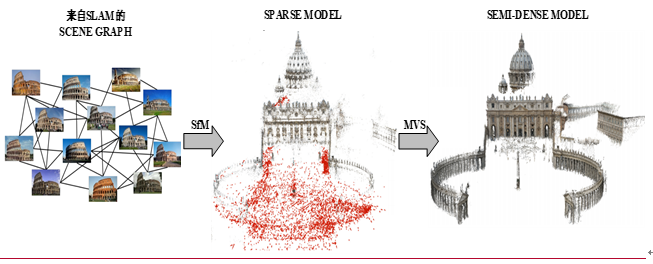
\includegraphics[height=6cm]{3d_constr_pipeline_sfm_mvs.png}
  \caption{离线3D重建技术流程图}
  \label{fig:3d_constr_pipeline_sfm_mvs}
\end{figure}
首先基于在线SLAM结果建立粗糙Scene Graph及点云环境地图,以全局大尺度地图及运动轨迹为优化目标,使用鲁棒性更高的特征描述算子,
利用高性能计算机的快速处理能力进行Global Bundle Adjustment全局优化,得到更加精确
的全局稀疏地图和运动轨迹。然后利用MVS(Multi View Stereo)技术对图像中的高梯度变化区域建立半稠密环境地图。